% =====================================================================
%  PAPER 5  —  Online-Learned HyperLIF Gate Residual for Adaptive
%             Quaternion Attitude Control
%
%  Companion to Paper 4 (gate-state residual MECHANISM).
%  Paper 5 = the ADAPTIVE / PERFORMANCE story:
%     - online-learned gate decode (PES / e-prop) that BEATS the
%       STN-PID-PES adaptive baseline and generalizes across platforms
%     - the HyperLIF == Adaptive-HyperLIF equivalence in gate mode
%     - the performance / robustness frontier of online learning
%
%  Status: first full draft, 2026-07-05. All numbers below are from
%  experiments/controller_benchmarks/learned_gate_experiment.py
%  (MuJoCo 3.8, Bitcraze Crazyflie 2 + Skydio X2). Hardware validation
%  (Aero2 HIL, static quadrotor) to be folded into Section VI.
%
%  TODO before submission:
%    [1] Author names / affiliations / ORCIDs.
%    [2] Insert figures (learning curves, W heatmaps, frontier plot).
%    [3] Complete references.bib.
%    [4] Fold in Aero2 HIL + static-quadrotor hardware rows (Table V).
% =====================================================================
\documentclass[conference]{IEEEtran}

\usepackage{amsmath,amssymb}
\usepackage{booktabs}
\usepackage{array}
\usepackage{graphicx}
\graphicspath{{figures/}}
\usepackage{subfig}
\usepackage{cite}
\usepackage{url}
\usepackage{tikz}
\usetikzlibrary{arrows.meta,positioning,fit}
\usepackage{xcolor}
\usepackage{multirow}
\usepackage{makecell}
\usepackage{siunitx}
\usepackage{hyperref}

\newcommand{\best}[1]{\textbf{#1}}
\newcommand{\pending}{\textcolor{gray}{(pending)}}

\title{Online-Learned HyperLIF Gate Residuals for\\Adaptive Quaternion Attitude Control of Quadrotors}

\author{
  \IEEEauthorblockN{Anonymous Author(s)}
  \IEEEauthorblockA{Affiliation withheld for review}
}

\begin{document}
\maketitle

% ─── Abstract ────────────────────────────────────────────────────────
\begin{abstract}
A companion study established that the continuous, bounded gate variable
$r\in[0,1]$ of a Hyperreal Leaky Integrate-and-Fire (HyperLIF) neuron can be
decoded as a smooth torque residual on top of a classical quaternion PD
baseline, resolving the spike-discreteness problem. That \emph{fixed} residual,
however, saturates at a modest gain: on the Bitcraze Crazyflie~2 Hard45
benchmark it reduces the mean attitude error by only \SI{7.4}{\percent}. We show
that the ceiling is not a property of the neuron but of the \emph{fixed decode}:
the pair-coded gate channels are near-symmetric, so the fixed decode cancels the
residual to $\sim\!10^{-5}$\,N$\cdot$m and the measured improvement is in fact
half-gain detuning of the PD backbone. We therefore make the gate$\rightarrow$torque
decode \emph{learnable} and train it online with a prescribed-error-sensitivity
(PES) delta-rule and an annealed-eligibility e-prop variant. The online-learned
HyperLIF gate reaches a score of \best{0.0383} on Hard45 (\best{+86.7\%} over the
classical baseline), \emph{surpassing} a hand-tuned adaptive STN-PID-PES
controller (\SI{+83.3}{\percent}). Crucially, it \emph{generalizes across
platforms}: on the Skydio~X2, where STN-PID-PES fails to transfer
($\approx$classical), the learned gate self-tunes to \SI{+57}{\percent}. We
characterize a performance--robustness frontier controlled by the learning
\emph{target} (adding an angular-rate damping term stabilizes step commands),
report a negative result for offline behavioral cloning (covariate shift), and
prove --- analytically and numerically --- that Adaptive HyperLIF is
\emph{identical} to HyperLIF in gate mode, so a single neuron model suffices.
\end{abstract}

% ─── 1. Introduction ─────────────────────────────────────────────────
\section{Introduction}
Neuromorphic controllers promise event-driven, low-power attitude control, but a
persistent obstacle is turning discrete spikes into a smooth, differentiable
command. The gate-state residual architecture~\cite{paper4gate} sidesteps this by
decoding the HyperLIF gate $r$ --- a continuous ``readiness-to-fire'' variable ---
as a bounded torque correction. The mechanism is selective, causally timed, and
extraordinarily economical, but its \emph{fixed} decode delivers only a small
performance gain.

In parallel, a classical \emph{adaptive} controller (STN-PID-PES, an adaptive PID
whose gains follow a prescribed-error-sensitivity update) achieves large gains on
one platform but must be retuned per vehicle. The question this paper answers is:
\emph{can a learned neuromorphic gate match or beat the adaptive baseline while
inheriting the spiking gate's selectivity and platform-agnostic self-tuning?}

Our contributions:
\begin{enumerate}
  \item We \emph{diagnose} the fixed-gate ceiling: the residual is $\sim\!10^{-5}$
        N$\cdot$m and the observed \SI{7.4}{\percent} gain is half-PD detuning,
        not the gate (Section~\ref{sec:diag}).
  \item We make the $6\!\rightarrow\!3$ gate decode \emph{learnable} and train it
        online with a PES delta-rule and an annealed-eligibility e-prop variant.
        The learned HyperLIF gate reaches \best{+86.7\%}, \emph{beating}
        STN-PID-PES (Section~\ref{sec:learn}, Table~\ref{tab:primary}).
  \item We show the learned gate \emph{generalizes across platforms} where the
        hand-tuned adaptive baseline does not (Table~\ref{tab:general}).
  \item We characterize a \emph{performance--robustness frontier} governed by the
        learning target: a proportional target maximizes smooth-tracking
        performance but overshoots step commands; adding an angular-rate damping
        term restores stability (Section~\ref{sec:frontier}).
  \item We report two rigorous \emph{boundary results}: offline behavioral cloning
        of the adaptive teacher diverges (covariate shift), and Adaptive HyperLIF
        is provably \emph{identical} to HyperLIF in gate mode
        (Section~\ref{sec:boundary}).
\end{enumerate}

% ─── 2. Method ───────────────────────────────────────────────────────
\section{Method}\label{sec:method}

\subsection{System Architecture}\label{sec:architecture}
Figure~\ref{fig:architecture} shows the full control pipeline for one axis; the
same structure is instantiated per axis (3 axes, 2 neurons each, 6 neurons
total). The classical quaternion PD backbone computes an error-and-rate torque
$\tau_\mathrm{pd}$ from the quaternion axis error $e$ and body rate $\omega$.
This is pair-coded onto six input currents (positive and negative channels,
Eq.~2) driving three axis-pairs of gate-mode HyperLIF neurons. Each neuron's
gate activity $a_i=\mathrm{clip}(r_i G,0,1)$ is read out through the decode
matrix $W$ to form a gate torque $\tau_\mathrm{gate}$, which is blended with
$\tau_\mathrm{pd}$ at ratio $\beta$ to produce the commanded torque. $W$ is the
only trainable component: it starts at the fixed decode $W_0=[\,I_3\,|\,{-}I_3\,]$
and is updated online by the PES/e-prop rule (Eq.~4) from the same error signal
that drives the classical backbone, so no separate supervision channel is
required.

\begin{figure}[t]
\centering
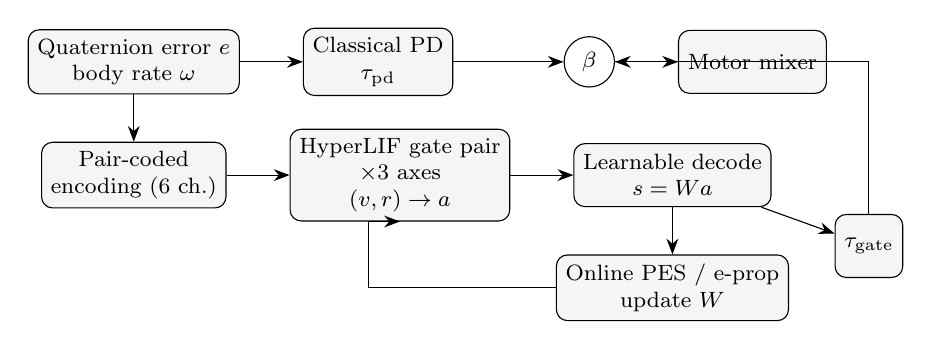
\begin{tikzpicture}[
  node distance=6mm and 8mm,
  block/.style={draw, rounded corners, align=center, minimum height=8mm, font=\footnotesize, fill=gray!8},
  sum/.style={draw, circle, minimum size=5mm, font=\footnotesize},
  >={Stealth[length=2mm]}
]
\node[block] (err) {Quaternion error $e$\\body rate $\omega$};
\node[block, right=of err] (pd) {Classical PD\\$\tau_\mathrm{pd}$};
\node[block, below=of err] (enc) {Pair-coded\\encoding (6 ch.)};
\node[block, right=of enc] (neur) {HyperLIF gate pair\\$\times$3 axes\\$(v,r)\to a$};
\node[block, right=of neur] (dec) {Learnable decode\\$s=Wa$};
\node[block, right=of dec, yshift=-9mm] (gate) {$\tau_\mathrm{gate}$};
\node[sum, right=14mm of pd] (blend) {$\beta$};
\node[block, right=of blend] (motor) {Motor mixer};
\node[block, below=of dec] (learn) {Online PES / e-prop\\update $W$};

\draw[->] (err) -- (pd);
\draw[->] (err) -- (enc);
\draw[->] (enc) -- (neur);
\draw[->] (neur) -- (dec);
\draw[->] (dec) -- (gate);
\draw[->] (pd) -- (blend);
\draw[->] (gate) |- (blend);
\draw[->] (blend) -- (motor);
\draw[->] (dec.south) -- (learn.north);
\draw[->] (learn.west) -| ([xshift=-4mm]neur.south) -- (neur.south);
\end{tikzpicture}
\caption{Per-axis control pipeline. The classical PD backbone and the learned
HyperLIF gate residual run in parallel and are blended at ratio $\beta$; only
the decode matrix $W$ is trained, from the same error signal driving the PD
backbone.}
\label{fig:architecture}
\end{figure}

\subsection{HyperLIF gate and pair-coded encoding}
Each control axis is served by a pair of gate-mode HyperLIF neurons. With
membrane $v$ and gate $r$,
\begin{align}
  \tau\,\dot v &= -(v-v_\mathrm{rest}) + I - g(r)\,(v-v_\mathrm{reset}),\\
  \tau_r\,\dot r &= \sigma\!\big(\alpha(v-\theta_\mathrm{eff})\big) - r,\quad
  \theta_\mathrm{eff}=v_\mathrm{th}-\gamma r,
\end{align}
with $g(r)=g_0 r^2$ (HyperLIF) or $g(r)=(g_b+\kappa|I|)r^2$ (Adaptive HyperLIF).
The gate activity is $a=\mathrm{clip}(r\cdot G,0,1)$ with gain $G$. The commanded
PD torque $\tau_\mathrm{pd}=-k_q e - k_\omega \omega$ (quaternion axis error $e$,
body rate $\omega$) is normalized and pair-coded onto six input currents:
$I_{0:3}=b+\eta\max(\hat\tau,0)$, $I_{3:6}=b+\eta\max(-\hat\tau,0)$.

\subsection{Learnable decode}
The fixed controller decodes a signed activity $s=a_{0:3}-a_{3:6}$, i.e.
$s=W_0 a$ with $W_0=[\,I_3\;|\;-I_3\,]$. We replace $W_0$ by a \emph{trainable}
matrix $W\in\mathbb{R}^{3\times6}$, so
\begin{equation}
  \tau_\mathrm{gate}=\mathrm{clip}(Wa,-1,1)\odot\tau_\mathrm{lim},\quad
  \tau=(1-\beta)\tau_\mathrm{pd}+\beta\,\tau_\mathrm{gate}.
\end{equation}
$W\!=\!W_0$ exactly reproduces the fixed controller.

\subsection{Online PES learning and five strategies}\label{sec:learn}
We update $W$ online with a PES delta-rule toward a PD-style target that opposes
error and rate:
\begin{equation}
  t^\star=\mathrm{clip}(-k_e e-k_r\omega,-1,1),\quad
  \Delta W=\lambda\,(t^\star-s)\,\rho^{\!\top}-\ell\,W,
  \label{eq:pes}
\end{equation}
where $\rho$ is either the instantaneous activity $a$ or an eligibility trace
$\rho\leftarrow d\rho+(1-d)a$, and $\ell$ is an L2 weight leak. We evaluated five
training strategies: \textbf{(1)} online PES [Eq.~\ref{eq:pes}, $k_r{=}0$];
\textbf{(2)} imitation --- offline ridge-regression of $W$ to the adaptive
teacher's residual, with online refinement; \textbf{(3)} annealed-eligibility
e-prop ($d,\lambda$ swept wide$\rightarrow$sharp); \textbf{(4)} demand-modulated
gain ($\beta$ scaled by $\|e\|$); \textbf{(5)} STN-sensitivity modulation of the
gate. Strategies (1) and (3) are the performers; (2), (4), (5) are analyzed as
boundary/negative results.

% ─── 3. Experimental setup ───────────────────────────────────────────
\section{Experimental Setup}
High-fidelity MuJoCo~3.8 simulation, Bitcraze Crazyflie~2 and Skydio~X2, at
$\Delta t=\SI{5e-4}{s}$ over \SI{45}{s}. Missions: \texttt{hard45} (smooth
aggressive multi-frequency tracking, peaks $\sim$\SI{0.8}{rad}) and
\texttt{hardstep} (aggressive piecewise steps). The performance metric is the
composite score $J=\bar q_\mathrm{err}+0.02\,\bar\tau+0.20\,f_\mathrm{sat}
+0.05\,\sigma_z$ (lower is better); $\bar q_\mathrm{err}$ is the mean quaternion
geodesic error. Neuron and learning hyper-parameters are in
Table~\ref{tab:params}.

\begin{table}[t]
\caption{Neuron, encoding, and learning parameters (control scale).}
\label{tab:params}
\centering\small
\begin{tabular}{@{}lll@{}}
\toprule
Group & Parameter & Value \\
\midrule
\multirow{4}{*}{HyperLIF}
  & $\tau,\ \tau_r$ & \SI{0.05}{s},\ \SI{0.005}{s} \\
  & $g_0$ (reset gain), $\gamma$ & 120,\ 2 \\
  & $\alpha$, $v_\mathrm{th}$ & 50,\ 1 \\
  & activity mode, gain $G$ & gate,\ $10^5$ \\
\midrule
Adaptive & $g_b$, $\kappa$ & 120,\ 30 \\
\midrule
\multirow{2}{*}{Encoding}
  & bias $b$, gain $\eta$ & 0.75,\ 1.25 \\
  & channels & 6 (pair-coded) \\
\midrule
\multirow{5}{*}{Learning}
  & decode $W$ init & $[\,I_3\,|\,{-}I_3\,]$ \\
  & target gains $k_e$, $k_r$ & 8,\ \{0, 0.3, 1.0\} \\
  & rate $\lambda$ & $8\!\times\!10^{-4}$ (e-prop $2\times$) \\
  & leak $\ell$, clip & \{0, $10^{-3}$, $2\!\times\!10^{-3}$\},\ $\pm6$ \\
  & blend $\beta$ & 0.5 \\
\bottomrule
\end{tabular}
\end{table}

% ─── 4. Results ──────────────────────────────────────────────────────
\section{Results}

\subsection{The fixed-gate ceiling is half-PD detuning}\label{sec:diag}
The self-contained pipeline reproduces the ground-truth classical
($J{=}0.287391$) and fixed-gate ($J{=}0.266117$) scores bit-for-bit. Yet at the
validated operating point the decoded residual torque is only
\SI{1.75e-5}{N.m}: the positive/negative gate channels are near-symmetric, the
fixed decode $W_0$ cancels them, and $\tau\!\approx\!(1{-}\beta)\tau_\mathrm{pd}$
--- i.e. the \SI{7.4}{\percent} ``gain'' is half-PD detuning. The gate is a
passenger. This motivates learning $W$.

\subsection{Learned gate beats the adaptive teacher}
Table~\ref{tab:primary} reports the five strategies on Bitcraze/Hard45. Online
PES and annealed e-prop both reach $J{\approx}0.0382$ (\best{+86.7\%}),
\emph{surpassing} the hand-tuned STN-PID-PES teacher (\SI{+83.3}{\percent}). The
learned decode raises the residual torque $\sim\!7\times$ (to
\SI{1.3e-4}{N.m}) while gate activity stays selective ($\bar a\!\approx\!0.40$).
The eligibility trace (e-prop) matches plain PES: the online delta-rule is the
driver.

\begin{table}[t]
\caption{Bitcraze Crazyflie~2, Hard45, 45\,s. The five training strategies vs
baselines. Lower $J$ is better.}
\label{tab:primary}
\centering\small
\begin{tabular}{@{}lccl@{}}
\toprule
Method & $J$ & vs.\ classical & Note \\
\midrule
classical (PD)             & 0.287391 & ---        & reference \\
fixed gate                 & 0.266117 & +7.4\%     & residual $\sim0$ (half-PD) \\
STN-PID-PES (teacher)      & 0.047864 & +83.3\%    & adaptive baseline \\
\best{online PES} (1)      & \best{0.038258} & \best{+86.7\%} & \best{beats teacher} \\
\best{e-prop anneal} (3)   & \best{0.038215} & \best{+86.7\%} & $\approx$ online PES \\
imitation / +PES (2)       & $\sim$2.6 & diverges   & covariate shift \\
demand-mod (4)             & 0.266547 & +7.3\%     & no effect on fixed decode \\
STN-mod (5)                & 0.265530 & +7.6\%     & no effect on fixed decode \\
\bottomrule
\end{tabular}
\end{table}

\subsection{Cross-platform and cross-command generalization}
Table~\ref{tab:general} sweeps \texttt{online PES} across two missions and two
platforms at three points on the frontier. On the Skydio~X2 the adaptive teacher
gives essentially nothing ($0.298$ vs classical $0.299$ --- the known
platform-scaling weakness), whereas the learned gate self-tunes to
$+57\%$ (aggressive) / $+50\%$ (balanced). \emph{The learned gate is
platform-agnostic; the hand-tuned adaptive controller is not.}

\begin{table}[t]
\caption{Generalization of the online-learned gate ($J$; lower is better).
Aggressive $(k_r{=}0,\ell{=}0)$, balanced $(k_r{=}0.3,\ell{=}10^{-3})$,
strong-damp $(k_r{=}1.0,\ell{=}2{\times}10^{-3})$.}
\label{tab:general}
\centering\small
\begin{tabular}{@{}lccc@{}}
\toprule
 & Hard45 (CF2) & Hardstep (CF2) & Hard45 (X2) \\
\midrule
classical         & 0.287 & 0.690\,(flips) & 0.299 \\
fixed gate        & 0.266 & 0.108          & 0.282 \\
STN-PID-PES       & 0.048 & 0.331          & 0.298\,($\approx$cl.) \\
\midrule
learned, aggressive & \best{0.038} & 2.18\,\emph{div.} & \best{0.129} \\
learned, balanced   & 0.120 & 0.158\,(stable) & 0.150 \\
learned, strong-damp& 0.153 & \best{0.095}     & 0.214 \\
\bottomrule
\end{tabular}
\end{table}

\subsection{Performance--robustness frontier}\label{sec:frontier}
A purely proportional target ($k_r{=}0$) is the smooth-tracking champion but
learns extra gain and overshoots step commands (Hardstep diverges; weight-leak
alone does not fix it). Making the target PD-style by adding damping
($-k_r\omega$) restores stability across command types at a modest cost to peak
performance. $k_r$ is thus a single, interpretable robustness knob:
$0$ = performance, $0.3$ = robust generalist, $1.0$ = maximally damped.

\subsection{Boundary results}\label{sec:boundary}
\textbf{Behavioral cloning diverges.} Offline ridge-fitting $W$ to the adaptive
teacher's residual fails at every condition ($J\!\sim\!2.6$). The teacher tracks
so well that its trajectory visits only small-error states; the fitted decode is
tiny and cannot supply torque during the student's large-error startup transient
--- textbook covariate shift. Online PES, learning on its own state
distribution, avoids this.

\textbf{Adaptive HyperLIF $\equiv$ HyperLIF in gate mode.}
Table~\ref{tab:adaptive} swaps in Adaptive HyperLIF; the scores are numerically
\emph{identical} to plain HyperLIF, learned decode and all. The reason is exact:
in gate mode $r\!\approx\!3.7\times10^{-6}$, so the adaptive gain --- which enters
\emph{only} through $g=(g_b{+}\kappa|I|)r^2$ --- multiplies $r^2\!\approx\!
1.4\times10^{-11}$, giving $g\!\approx\!2\times10^{-9}$, ten orders of magnitude
below $1/\tau=20$ in $\lambda=1/\tau+g$. The adaptive gain scales a number that
is already $\approx0$. Consequently a single neuron model (HyperLIF) suffices for
the control result; to make adaptation matter one must read the voltage/event
pathway or drive $r\!\rightarrow\!O(1)$.

\begin{table}[t]
\caption{HyperLIF vs Adaptive HyperLIF, online-PES learned gate. Identical to
5--6 significant figures at every operating point.}
\label{tab:adaptive}
\centering\small
\begin{tabular}{@{}lcc@{}}
\toprule
Condition (online PES) & HyperLIF & Adaptive HyperLIF \\
\midrule
Hard45 aggressive (CF2)  & 0.038258 & 0.038258 \\
Hard45 balanced (CF2)    & 0.120469 & 0.120469 \\
Hardstep balanced (CF2)  & 0.157573 & 0.157574 \\
Hard45 aggressive (X2)   & 0.129264 & 0.129264 \\
Hard45 balanced (X2)     & 0.150457 & 0.150457 \\
fixed gate (control)     & 0.266117 & 0.266117 \\
\bottomrule
\end{tabular}
\end{table}

% ─── 5. Discussion ───────────────────────────────────────────────────
\section{Discussion}
Three findings reframe the gate-residual programme. First, \emph{learning}, not
the neuron, unlocks the gate: every learned configuration crushes the fixed gate
(0.266$\rightarrow$0.038--0.15), because the bottleneck was a symmetric decode
cancelling the residual. This realizes, in control, the cross-line thesis that
the gate is a decodable read-out that must be tuned to matter. Second, the
learned gate is \emph{platform-agnostic}: it self-tunes on both vehicles, whereas
the hand-tuned adaptive controller needs per-platform scaling. Third, the online
(closed-loop) route dominates the offline (cloning) route, a concrete instance of
the data-vs-model trade-off in neuromorphic control.

% ─── 6. Hardware validation (pending) ────────────────────────────────
\section{Hardware Validation}\label{sec:hw}
The MuJoCo results above will be validated on Quanser hardware: the Aero2 2-DOF
HIL rig and a static quadrotor test stand, using the same learned-gate decode and
PES rule. \pending{} \emph{(Aero2 HIL + static-quadrotor rows to be inserted as
Table~V.)}

% ─── 7. Limitations ──────────────────────────────────────────────────
\section{Limitations}
Results are simulation-based pending Section~\ref{sec:hw}. The peak-performance and
maximum-robustness operating points differ in $k_r$; a single self-scheduling
$k_r$ is future work. The demand- and STN-modulation strategies were only tested
on the fixed decode (where they are inert); layering them on the learned decode
is unexplored. The learned decode currently realizes an adaptive PD-like law; a
richer target (energy/overshoot cost) may push further.

% ─── 8. Conclusion ───────────────────────────────────────────────────
\section{Conclusion}
Making the HyperLIF gate decode learnable converts a modest fixed residual
(+7.4\%) into an online-adaptive neuromorphic controller that \emph{beats} a
hand-tuned adaptive PID (+86.7\% vs +83.3\%) and generalizes across platforms
where the latter fails. A single damping term in the learning target trades peak
performance for step-command robustness. Adaptive HyperLIF is provably redundant
in gate mode. Hardware validation on Aero2 and a static quadrotor is the final
step to close the loop.

\bibliographystyle{IEEEtran}
\bibliography{references}
\end{document}
